\documentclass[a4paper]{article}
\usepackage[utf8]{inputenc} 
\usepackage[T1]{fontenc}
\usepackage{lmodern}
\usepackage{graphicx}
\usepackage[french]{babel}
\usepackage{csquotes}
\usepackage{listings}
\usepackage{float}
\usepackage{geometry}
\geometry{hmargin=2.5cm,vmargin=1.5cm}
\usepackage[citestyle=authortitle,defernumbers=true]{biblatex}
\addbibresource{bibliographie.bib}
\usepackage{color}
\usepackage{pdfpages}
\definecolor{lightgray}{rgb}{.9,.9,.9}
\definecolor{darkgray}{rgb}{.4,.4,.4}
\definecolor{purple}{rgb}{0.65, 0.12, 0.82}
\lstdefinelanguage{JavaScript}{
  keywords={break, case, catch, continue, debugger, default, delete, do, else, false, finally, for, function, if, in, instanceof, new, null, return, switch, this, throw, true, try, typeof, var, void, while, with},
  morecomment=[l]{//},
  morecomment=[s]{/*}{*/},
  morestring=[b]',
  morestring=[b]",
  ndkeywords={class, export, boolean, throw, implements, import, this, number, string},
  keywordstyle=\color{blue}\bfseries,
  ndkeywordstyle=\color{darkgray}\bfseries,
  identifierstyle=\color{black},
  commentstyle=\color{purple}\ttfamily,
  stringstyle=\color{red}\ttfamily,
  sensitive=true
}

\lstset{
   language=JavaScript,
   backgroundcolor=\color{lightgray},
   extendedchars=true,
   basicstyle=\footnotesize\ttfamily,
   showstringspaces=false,
   showspaces=false,
   numbers=left,
   numberstyle=\footnotesize,
   numbersep=9pt,
   tabsize=2,
   breaklines=true,
   showtabs=false,
   captionpos=b
}
\nocite{*}
\newcommand{\lexique}[2]{\item{\textbf{#1}:} #2}
\renewcommand{\lstlistingname}{Figure}% Listing -> Algorithm
\newcommand{\img}[3][]{
    \begin{figure}[H]
        \centering
        \includegraphics[width=#3\textwidth]{#2}
        \caption{#1}    
    \end{figure}
}
\newcommand{\inlinecode}[1]{\colorbox{lightgray}{#1}}
\newcommand{\ptitle}[1]{\vspace{10pt}
{\large \noindent \textbf{#1}}}

\author{Torrenté Florian}
\title{Travail de maturité - Puissance4IA}

\begin{document}
\maketitle

\tableofcontents

\newpage
\section{Introduction}

\subsection{Problématique et objectifs}
    Dans quelle mesure l'implémentation d'une intelligence artificielle pour jouer au Puissance 4 est-elle compliquée, et quelles en sont les difficultés ?

    Dans ce travail, je voulais renforcer mes connaissances sur les différents langages webs (HTML, CSS3 et JavaScript) mais surtout me rapprocher du domaine de l'intelligence artificielle qui a l'air d'être un sujet très prometteur pour le futur. En clair, les objectifs de ce travail étaient:
    \begin{enumerate}
        \item Comprendre le fonctionnement d'une intelligence artificielle
        \item Développer un ou plusieurs algorithmes
        \item Comprendre les limites de ces algorithmes et essayer de les dépasser
        \item Créer une intelligence que je ne pourrai plus battre au Puissance 4
    \end{enumerate}

\subsection{Description et règles du jeu}
    Le Puissance 4 est un jeu avec des règles très simples. Le but du jeu est d'aligner quatre pions de même couleur (horizontalement, verticalement, ou en diagonale). Le terrain de jeu est une grille de 7x6 (sept colonnes et six lignes). Chaque joueur possède des pions d'une couleur (généralement jaune et rouge). Chacun son tour, les joueurs déposent un pion dans la colonne de leur choix, le pion descend alors le plus bas possible dans la colonne. Le premier joueur à aligner quatre pions de sa couleur gagne. S'il n'y a plus de place pour jouer, la partie est nulle.


    \img[Un exemple de partie gagnée par le joueur rouge.]{Images/puissance4.jpg}{0.5}

    Les règles sont résolument simples, mais il y a une raison supplémentaire pour laquelle j'ai choisi ce jeu: c'est un jeu à information complète. Cela veut dire que chaque joueur connait : \begin{itemize}
        \item tous les coups qu'il peut jouer;
        \item tous les coups que son adversaire peut jouer;
        \item les gains résultants de ces actions;
        \item le but de l'autre joueur.
    \end{itemize}
    Ces différentes conclusions permettent d'utiliser des algorithmes comme \textit{Minimax}, qui sont conçus pour minimiser les pertes. Pour ce faire on a besoin des différentes informations du jeu, en effet, si de l'aléatoire intervenait dans les règles du jeu, il serait impossible d'implémenter ce genre d'algorithmes.

\subsection{L'intelligence artificielle}
    L'humanité s'est donné le nom scientifique \textbf{homo sapiens}---l'homme sage---parce que nos capacités mentales sont extrêmement importantes pour nous et notre sentiment d'identité. Le domaine de l'intelligence artificielle (ou IA) tente de comprendre cette intelligence. C'est pourquoi l'étudier peut nous permettre d'en apprendre davantage sur nous-même. Contrairement à la philosophie et à la psychologie, qui s'intéressent aussi à l'intelligence, l'IA essaye de \textit{construire} des entités intelligentes et de les comprendre. Une autre raison d'étudier l'IA est que ces entités construites sont intéressantes et utiles en elles-mêmes. En effet, ces dernières ont donné naissance à de nombreux résultats significatifs et impressionnants. On peut citer, par exemple, les intelligences artificielles pour la navigation (comme GoogleMaps ou Waze), la reconnaissance faciale, la correction et la traduction de texte et autre. C'est un domaine de l'informatique qui fait désormais partie de nos vies quotidiennes, mais reste assez peu connu par le grand public.

    Maintenant, nous savons pourquoi le domaine de l'IA est intéressant et important, nous avons toujours besoin de savoir précisément \textit{ce que c'est}. On pourrait simplement dire: "Eh bien, ce sont des programmes intelligents", mais je pense qu'il est important de bien définir ce qu'est l'intelligence et par extension l'intelligence artificielle avant de se lancer dans sa création. Une cohérente pour moi serait celle-ci: "L’intelligence artificielle a pour objectif de construire des dispositifs simulant les processus cognitifs humains"\footcite{haiech_2020}. En clair, des programmes qui permettent de résoudre des problèmes qui étaient, avant, exclusivement résoluble avec une intervention humaine.


\subsection{La structure des données}
    Pour implémenter un algorithme, il faut définir une structure de donnée très légère et optimisée afin de pouvoir calculer des milliers de positions de partie en quelques secondes. Pour comprendre cette structure de donnée, nous allons devoir plonger dans le fonctionnement des ordinateurs. Nous allons explorer: les \textit{bits}, leur manipulation et enfin les \textit{bitboards}.
    
    \ptitle{Les bits}
    Dans les ordinateurs, toutes les informations sont stockées sous forme de bits\footnote{De l'anglais \textit{binary digit}}. On peut voir un bit comme une boite contenant soit 0 soit 1. L'utilisation des bits est assez naturelle en informatique, car, conventionnellement, 0 est éteint et 1 allumé. Maintenant, on a cette boite, mais comment faire si on veut stocker autre chose que 0 ou 1 ? Avant de répondre à cette question, il nous faut examiner notre façon de compter. Dans la vie de tous les jours, nous comptons utilisons les nombres en base 10\footnote{Ou système décimal}. Cela veut dire qu'on utilise 10 chiffres différents pour écrire tous les nombres (0, 1, 2, 3, 4, 5, 6, 7, 8, 9). Pour compter, on incrémente la boite la plus à droite jusqu'à 9. Une fois à neuf, pour incrémenter encore, on incrémente la boite de gauche et on transforme le 9 en 0.
    
    \img[Comptage en base 10]{Images/ComptageDecimal.PNG}{0.5}

    Revenons à notre question: pour stocker autre chose que 0 ou 1, on utilise plusieurs bits pour compter en base 2. Au lieu d'avoir 10 chiffres, on n'en a que 2 : 0 et 1. L'écriture du nombre 3 en base 2 est donc : 11. Pour passer de base 2 à base 10, il faut numéroter nos boites de droite à gauche (en partant de 0) et appliquer cette formule (on notera $B_i$ le chiffre dans la boite i et n le nombre de boite): $\sum_{i=0}^{n} B_i\cdot2^{i}$. Par exemple 11 (en base 2) = $1\cdot2^{0}+1\cdot2^{1} = 3$.
     
    En informatique, un \textit{long integer} est composé de huit octets, c'est-à-dire 64 bits. On numérote les bits de ce nombre de droite à gauche (sans oublier qu'en informatique, on commence à compter à 0).

    \begin{lstlisting}
        63 62 61 60 ... 48 47 46 45 ... 3 2 1 0
    \end{lstlisting}
    
    Comme on l'a vu précédemment, le Puissance 4 se joue sur un \textit{board} vertical, avec sept colonnes et six lignes, ce qui fait 42 cases. Comme on peut le voir sur le diagramme ci-dessous, on ajoute une ligne en haut et deux colonnes à droite pour éviter les erreurs de saut lors des opérations pour la vérification de victoire. Cette représentation est appelée \textit{bitboard}
    \img[Représentation du bitboard]{Images/BitBoard.png}{0.7}
    Les nombres indiquent la position (l'\textit{index}) dans la représentation binaire d'un long. Par exemple, le 25 représente le 25ème bit de ce nombre. En clair, notre bitboard est simplement un nombre, qu'on représente en base 2, et qu'on place en 2 dimensions pour représenter le terrain de jeu.

    Comme le jeu est joué par deux joueurs, on utilisera un bitboard par joueur.
    Prenons un exemple en représentant cette position:
    \img[Partie en cours avec les bitboards]{Images/ExempleBitBoardsPt2.png}{0.7}
    On peut aussi le voir "à plat", en regroupant les bits par paquets de 7 (ce qui représente une colonne entière, c'est-à-dire avec la ligne supplémentaire) ce qui ressemble à ceci :
    \img[Représentation des bitboards "à plat"]{Images/FlatBiboard.png}{1}
    Cette représentation du board sera très pratique par la suite pour faire les opérations sur ces bits (les opérations seront plus simples à visualiser).

    Cette manière de représenter les états du jeu est la clé à la vitesse de la vitesse de l'algorithme. En effet, cette représentation permet en utilisant seulement des opérations de base, comme nous allons le voir ci-dessous, de jouer des coups, de tester s'il y a une victoire, une nulle, etc... Enfin, cette représentation est très légère et permet donc un stockage assez simple et demande très peu de RAM pour fonctionner.

    Maintenant qu'on a vu comment les boards sont représentés, on va pouvoir explorer comment on va traiter ces données, pour jouer des coups et tester s'il y a une victoire. Pour ce faire on n'a besoin que de deux types d'opérations: le \textit{bit shifting} (décalage de bit) et la combinaison de bit (notamment XOR et AND).

    \ptitle{Le décalage de bits}

    Pour décaler des bits en informatique, on utilise 2 opérateurs : \inlinecode{>>} et \inlinecode{<<}. Respectivement \textit{right shift} et \textit{left shift}. Par exemple \inlinecode{0b10101110 << 3} signifie que l'on retire les 3 premiers nombres à gauche et on ajoute 3 zéros à droite. Ici, le préfixe 0b indique que les chiffres suivants représentent un nombre binaire et non un nombre décimal. Donc \inlinecode{0b10101110 << 3 = 0b01110000}.
   
    De manière similaire, \inlinecode{0b10101110 >> 3 = 0b00010101}.

    
    \ptitle{La combinaison de bits}

    Les deux seuls opérateurs dont nous aurons besoin sont le \textit{XOR} et le \textit{AND}. L'opérateur XOR, ou OR exlusif, (qu'on écrit \inlinecode{\^{}}) prend deux nombres binaires, par exemple \inlinecode{0b10101110 \^{} 0b10011111}, et compare les bits de même position. Si les deux bits sont différents, le résultat est 1, sinon, c'est 0.

    Si on écrits les deux nombres l'un sur l'autre, les bits sont facile à comparer.
    \img[Exemple de l'opérateur XOR]{Images/XORExemple.png}{0.15}

    L'opérateur AND (qu'on écrit \inlinecode{\&}) prend aussi 2 nombres binaires et les compare bit par bit. Si les deux bits sont un 1, le résultat est 1, sinon 0.
    \img[Exemple de l'opérateur AND]{Images/ANDExemple.png}{0.15}

    Toutes ces différentes opérations vont être utilisées directement dans la partie suivante pour, entre autres, jouer un coup et vérifier si un joueur a gagné.

\subsection{Application des bitboards pour le puissance 4}

    Pour montrer l'utilisation des bitboards je vais vous présenter les 2 fonctions principales dont nous avons besoin : \inlinecode{makeMove} et \inlinecode{isWin}. La première permet de jouer un coup tandis que la seconde permet de déterminer si un joueur a gagné.

    Avant d'examiner ces fonctions, nous avons encore besoin de garder en mémoire : la position à remplir de chaque colonne qui sera stockée dans le tableau \inlinecode{heights} et la hauteur max de chaque colonne qui sera stockée dans le tableau \inlinecode{max\_heights}.

    \img[Début de partie]{Images/EmptyBoard.png}{0.4}

    Comme on le voit dans la figure ci-dessus, au début de la partie les hauteurs sont: \newline\inlinecode{heights = \{0, 7, 14, 21, 28, 35, 42\}} et les hauteurs max sont: \inlinecode{max\_heights = \{6,13,20,27,34,41,48\}}. À chaque fois qu'un coup sera joué dans une colonne, on augmentera l'indice de la colonne de 1. En gardant ceci en mémoire, cela nous évite de devoir chercher la prochaine case vide à chaque coup joué.

    \ptitle{Jouer un coup}

    \begin{lstlisting}
        function makeMove(column, playerBoard) {
            move = 1 << height[column]; // (1)
            playerBoard = playerBoard ^ move;  // (2)
            height[column] += 1; // (3)
        }
    \end{lstlisting}
    Voici ce que le code fait : 
    \begin{enumerate}
        \item On récupère la valeur height en fonction de la colonne donnée et on l'utilise pour décaler le nombre 1 vers la gauche jusqu'à cette position. Ensuite on stock cette valeur dans la variable \inlinecode{move}.
        \item On prend le board représentant le joueur et on utilise l'opérateur XOR avec la variable \inlinecode{move}. (\inlinecode{playerBoard \^{} move}) et on met à jour la nouvelle valeur du bitboard.
        \item On incrémente la valeur de la hauteur de cette colonne de 1 pour être prêt pour le prochain coup.
    \end{enumerate}

    Je pense qu'un exemple aidera à mieux visualiser la situation. Imaginons que je veux jouer un coup dans la colonne 3. Je vais donc chercher l'index de la hauteur de cette colonne : \inlinecode{heights[3]} qui vaut \inlinecode{21}. Je décale donc mon \inlinecode{1} 21 fois vers la gauche (\inlinecode{1 << 21}).

    \img[Exemple de la fonction makeMove]{Images/ExempleMakeMove.png}{1}

    % \newpage
    \ptitle{Est-ce qu'un joueur à gagné ?}

    Reprenons la représentation du bitboard :
    \img[Représentation du bitboard]{Images/BitBoard.png}{0.5}
    % Pour savoir s'il y a 4 pièces alignées horizontalement, on doit, par exemple, regarder si les positions 11, 18, 25 et 32 sont toutes des 1. On pourrait aussi regarder les positions 21, 28, 35 et 42. Le pattern là-dessous est simple: on prend la position la plus à gauche et on ajoute 7 à chaque fois.

    % Verticalement, ce nombre est 1 (par exemple les positions 15 et 16). En diagonale, ce nombre est soit 8 (par exemple 16 et 24) ou alors 6 (30 et 36).

    % Donc les nombres "magiques" sont 1, 6, 7 et 8.

    % Pour tester s'il y a 4 pièces alignées, on va prendre notre bitboard, faire une copie et la décaler à droite d'un de ces nombres, refaire une copie et la décaler de 2 fois plus et encore une copie, mais cette fois-ci 3 fois plus. Ensuite, on combine toutes les copies avec l'opérateur AND et le tour est joué. Si la réponse est différente de 0 alors il y a 4 pièces alignées.

    % Encore une fois, un exemple sera probablement plus clair:
    % \img[Exemple de la fonction isWin]{Images/ExempleIsWin.png}{0.8}

    Pour savoir si 4 pièces sont alignées horizontalement, on doit vérifier par exemple si les positions 11, 18, 25 et 32 sont toutes des 1. De la même manière, on pourrait vérifier les positions 21, 28, 35 et 42.

    \img[Exemple puissance 4 horizontal]{Images/CheckWinHorizontal.png}{0.5}

    En partant de n'importe quelle position et en sautant de 7 en 7, on peut vérifier s'il y a 4 pièces alignées. De manière similaire pour les puissances 4 verticaux et diagonaux :

    \img[Les chiffres "magiques"]{Images/MagicNumbers.png}{0.5}

    Ces chiffres "magiques" (magiques parce que grâce à ces 4 chiffres, on peut vérifier tous les alignements possibles sur le board) sont donc: 1, 6, 7, 8. Maintenant, en utilisant 2 opérateurs vus précédemment (AND et le \textit{right shift}) on va pouvoir vérifier toutes les possibilités très rapidement. Avec les shifts, on va aligner les positions correspondantes (en shiftant les chiffres magiques 1x, 2x et 3x). Une fois alignés, on les combine avec l'opérateur AND. Si le résultat est différent de 0, alors il y a 4 pièces alignées.

    \img[Exemple de la fonction isWin]{Images/ExempleIsWin.png}{0.8}

    \newpage
    Maintenant que nous savons comment ça marche, il suffit de l'implémenter pour toutes les directions. Le symbole \inlinecode{!=} signifie "différent de".
    \begin{lstlisting}
    isWin(bitboard) {
        if (bitboard & (bitboard >> 6) & (bitboard >> 12) & (bitboard >> 18) != 0) return true; // diagonal \
        if (bitboard & (bitboard >> 8) & (bitboard >> 16) & (bitboard >> 24) != 0) return true; // diagonal /
        if (bitboard & (bitboard >> 7) & (bitboard >> 14) & (bitboard >> 21) != 0) return true; // horizontal
        if (bitboard & (bitboard >> 1) & (bitboard >>  2) & (bitboard >>  3) != 0) return true; // vertical
        return false;
    }
    \end{lstlisting}

    Par direction, la fonction a besoin d'environ 7 opérations : 3 shifts, 3 AND et 1 comparaison. Une évaluation complète du board requiert donc 4x7=28 opérations. Les ordinateurs actuels effectuent environ 3 milliards d'opérations par seconde, on peut donc évaluer environ \textbf{100 millions de positions par seconde}.

\section{Déroulement du travail}

\subsection{Structure et technologies}

	Le projet est divisé en 2 parties principales: le \textit{client} et le \textit{serveur}. Le premier contient tout ce que l'utilisateur verra (la page internet, le jeu) et gérera toutes les interactions avec ce dernier. Toutes les informations du client sont ensuite traitées par le serveur à distance. C'est donc le serveur qui sera en charge de calculer les coups de l'IA et de les envoyer au client. Cette structure permet entre autres d'avoir une interface client très légère et donc utilisable sur tous les appareils. Le problème est que la charge de calcul est entièrement sur le serveur, ce qui peut poser problème si beaucoup d'utilisateurs voulaient affronter l'IA.

	Pour tout le projet, j'utilise NPM (pour  "\textit{Node Package Manager}") qui permet de gérer les dépendances de mon projet simplement. Toutes les informations pour NPM sont contenues dansun fichier \textit{package.json}. On y trouve: la description du projet (nom, description, version, auteur, etc...), les différents scripts (raccourcis pour lancer, générer le projet) et les dépendances.

    \ptitle{Le client}

	\noindent Dans le dossier client se trouve:
	\begin{enumerate}
		\item Le dossier css
		\item Le dossier js
		\item index.html
		\item package.json
	\end{enumerate}
    \vspace{5pt}

	(1) Le dossier CSS (pour \textit{"Cascading StyleSheet"}) contient les feuilles de style qui permettent de modifier l'apparence de ma page web. Pour ce projet, j'ai décidé de ne pas utiliser le langage CSS, mais de passer par SASS (Syntactically Awesome Stylesheets). Ce langage permet d'écrire un code plus visuel et pratique qui sera ensuite compilé en CSS.

	(2) Le dossier JS (pour \textit{JavaScript}) contient toute la logique de la page. En effet, le JavaScript est un langage qui permet de rendre une page web dynamique et d'y dessiner ce qu'on veut (comme par exemple un jeu du puissance 4). Pour dessiner le plateau de jeu, j'utilise la librairie \textit{p5js} qui gère de manière élégante et légère toutes les actions de dessins et les interactions avec l'utilisateur. Pour ce projet, j'ai aussi décidé d'utiliser \textit{TypeScript} qui est un langage (qui se compile en JavaScript) permettant d'avoir un code plus prévisible et d'attraper les erreurs plus tôt.

	(3) Le fichier \textit{index.html} contient simplement la structure de la page et charge le css et le js.

	(4) Le \textit{package.json} contient les informations pour NPM, permettant notamment d'automatiser la compilation du TypeScript et du SASS, ainsi que l'installation de p5js.

	En résumé, pour le client j'utilise 3 langages (HTML, SASS et TypeScript), la librairie p5js et le gestionnaire de paquet NPM.

    \ptitle{Le serveur}

	\noindent Le dossier serveur quant à lui contient:
	\begin{enumerate}
		\item Le dossier src
		\begin{enumerate}
            \item Bitboard.ts
            \item AI.ts
            \item index.ts
        \end{enumerate}
		\item package.json
	\end{enumerate}
    \vspace{5pt}

	(1) Le dossier \textit{src} (abréviation de \textit{source}, comme "code source") contient toute la logique du serveur. Tout le code qu'il contient est écrit en TypeScript. Il contient 3 fichiers:
	    
	\indent\indent(a) Le fichier Bitboard.ts (\textit{ts} est l'extension des fichiers contenant du code TypeScript) qui contient l'implémentation des bitboards.

	\indent\indent(b) Le fichier AI.ts qui contient toute la logique de l'intelligence artificielle

	\indent\indent(c) Enfin, l'index.ts contient la logique pour recevoir et envoyer des informations au client.

	(2) Le package.json contient, comme vu précédemment, toutes les informations pour le gestionnaire de paquets NPM.

\subsection{Implémentation du client}    

    Dans cette section, je vais survoler l'implémentation du client, son évolution et les différents problèmes que j'ai pu rencontrer.

    Pour commencer, le client étant une page web, j'ai créé le \inlinecode{index.html}. Ce fichier appelé "index", par convention, contient la structure de notre page. C'est aussi ce fichier qui va regrouper la structure, le code Javascript et le style. En réalité, sa structure est extremement simple, elle contient simplement quelques informations, et un endroit préparé pour afficher le jeu.

    Les deux fichiers les plus importants du client sont le fichier \inlinecode{sketch.ts} et \inlinecode{connect4.ts}. A eux deux, ils gèrent tout le jeu et les intéractions avec l'utilisateur.

    A l'origine, la page ressemblait à ceci:
    \img[Première version du client]{Images/FirstClientPreview.png}{0.8}

    Ce n'était pas très beau, pas très ergonomique et pas dynamique du tout. Mais cela suffisait pour mes tests. Après quelques temps j'ai décidé de changer tout cela, et de donner une look plus moderne à mon travail. Voici ce à quoi la page ressemble maintenant :
    \img[Deuxième version du client]{Images/SecondClientPreview.png}{0.8}
    En plus d'être plus joli, il y a une animation quand les pièces tombent pour que cela soit plus agréable.

    En soit, dans l'implémentation, je n'ai rencontré presque aucun problème. En effet, j'étais habitué à développer ce genre de jeu, la seule nouveauté était le langage, car les navigateurs ne peuvent interagir avec TypeScript, j'ai donc dû trouver comment le compiler correctement afin que l'application marche sur tous les navigateurs. Pour ce faire, j'utilise simplement une libraire appelée \textit{Browserify} qui permet de compiler tout le projet et de le stocker dans un fichier unique.

\subsection{Implémentation des bitboards}

	L'implémentation des bitboards est résolument simple, grâce à une théorie claire et des opérations extrêmement simples. J'ai tout de même rencontré certains problèmes liés à des spécificités de JavaScript. Mais avant d'exposer ces problèmes, voyons l'implémentation.

	Comme vu dans la théorie, je commence par initialiser les constantes comme \newline\inlinecode{max\_heights = [5, 12, 19, 26, 33, 40, 47]} et \inlinecode{directions = [1, 6, 7, 8]} (les directions sont les chiffres "magiques" de la théorie). Je déclare aussi une variable \textit{data} qui contiendra les bitboards des deux joueurs et une variable \inlinecode{heights = [0, 7, 14, 21, 28, 35, 42]} qui gardera en mémoire la hauteur de chaque colonne. On prépare aussi une variable \inlinecode{counter = 0} qui permet de compter les coups joués (qui est aussi pratique, car s'il est pair, c'est au tour du joueur 1 sinon, c'est au tour du joueur 2). Enfin, on crée un tableau \textit{moves} qui gardera tous les coups en mémoire.

	Voyons ensemble, par exemple, la fonction \textit{move} en TypeScript:
	\begin{lstlisting}
move(column: number): void {
    let move = new Long(1).shl(this.heights[column]); // On recupere la hauteur stockee dans heights avec la colonne et on shift le 1 ce nombre de fois a gauche
    this.heights[column]++; // On incremente la hauteur de la colonne
    this.data[this.counter & 1] = this.data[this.counter & 1].xor(move); // On joue le coup sur le board
    this.moves[this.counter++] = column; // On enregistre le coup
}
	\end{lstlisting}

	(1) On voit \inlinecode{column: number}, cela permet d'indiquer que la variable \textit{column} est un nombre. On voit aussi \textit{: void}, ce qui indique que cette fonction ne retourne rien.
	
    (2) \textit{shl} est l'abréviation de \textit{shift left}.

	
	Un problème que je n'avais néanmoins pas anticipé, est que JavaScript stock ses nombres dans un espace qui fait $2^{52}$ bytes (ce qui limite leur taille à maximum $2^{52}$), mais lors de l'utilisation d'opérateurs sur les bits (comme le AND et les shifts), ces nombres sont limités à $2^{32}$, alors que dans certains cas, notre représentation du bitboard peut dépasser ce nombre. Il a donc fallu que j'utilise une librairie appelée \textit{long} qui permet elle de gérer les nombres jusqu'à $2^{64}$, ce qui est suffisant.

\subsection{Implémentation de minimax}

    Avant d'implémenter un algorithme connu, j'ai d'abord essayé beaucoup de choses, certaines marchaient mais étaient beaucoup trop lentes, certaines ne marchaient simplement pas. Après avoir essayé toutes ces choses, je me suis renseigné sur les algorithmes existants et ai dessidé d'utiliser celui-ci car il me semblait être le plus adapté. Mais avant de l'implémenter, voyons comment il fonctionne.
    
    Pour utiliser l'algorithme minimax sur un jeu, il faut que ce jeu soit \textit{un jeu non-coopératif synchrone à information complète opposant deux joueurs, [...] à somme nulle}\footcite{wiki_minimax_neuman}. En clair, un jeu ou deux joueurs s'affrontent, chacun leur tour, où chaque joueur connaît toutes les informations et où la somme de la perte et des gains des deux joueurs est nulle. Le Puissance 4 remplit toutes ces conditions tout comme les échecs (trop compliqués) et le morpion (trop simple). En théorie, l'algorithme fonctionne en 5 étapes : 
    \begin{enumerate}
        \item On génère tout l'arbre du jeu (voir ci-dessous), jusqu'en tout en bas aux positions finales (victoire ou nulle)
        \item On applique une \textit{heuristique}\footnote{Une heuristique est un nombre qui fournit, pas nécessairement de manière excacte, un score à une position.} à chaque position finale
        \item On détermine la valeur des nodes au dessus grâce à la valeur des nodes d'en dessous.
        \item On fait remonter ces valeurs d'étage en étage jusqu'en haut
        \item On choisi le chemin avec la plus grande valeur
    \end{enumerate}
    Pour les représenter, j'utiliserai des versions simplifiées (comme par exemple des plateaux de morpion), pour que les shémas restent lisibles.

    \img[Un arbre de recherche (partiel) du morpion]{Images/MinimaxShema.png}{0.8}
    
    On voit que sur les coups du joueur \textit{X}, on cherche la valeur maximale (max) et sur les coups de l'autre joueur, on cherche la valeur minimale (min). D'où le nom de l'algorithme: \textbf{minimax}. Une application sur un jeu encore plus trivial pourrait ressembler à ceci :
    \img[Exemple de mininax]{Images/MinimaxShema2.png}{0.75}
    On voit que ce jeu se termine après le deuxième coup. Maintenant, pour déterminer le meilleur coup pour le premier joueur, il faut "remonter" les valeurs jusqu'en haut pour voir quel chemin est le plus rentable. La dernière ligne est une ligne impaire (donc min), on cherche donc la plus petite valeur entre les 3 de chaque node. Pour B1, ça sera 3, pour B2, ça sera 2 et pour B3, ça sera 1. Maintenant pour A on cherche le maximum entre les 3 en dessous, c'est-à-dire 3. Donc le meilleur chemin est A -> B1 -> C3.
    \img["Remontée" des valeurs]{Images/MinimaxShema3.png}{0.6}

    Cet algorithme est en théorie infaillible. En effet, si l'on atteint la fin de l'arbre il suffit de jouer le meilleur coups à chaque fois pour gagner. Mais calculer toutes ces positions à chaque coups est beaucoup trop long. En effet, une estimation du nombre de positions possibles au Puissance 4 est d'environ \textbf{$1.6\cdot10^{13}$} positions. Même si on a estimé qu'avec les bitboards on pouvait calculer environ 100 millions de positions par seconde (en réalité probablement beaucoup moins), il faudrait au minimum 44h et 25 minutes pour calculer 1 coup\footnote{Le calcul est le suivant: $1.6\cdot10^{13}\div10^{8} = 1.6\cdot10^{5}$ secondes. Soit 44h 26min et 40sec. A noter que cette valeur serait pour un ordinateur entièrement consacré à ce calcul, avec un language plus optimisé que le JavaScript.}. Il a donc fallu trouver des moyens pour palier à ce problème.

\subsection{Optimisations de l'algorithme}

    Pour améliorer et rendre plus viable l'algorithme, j'y ai appliqué 3 modifications. Les deux premières pour gagner du temps, et la dernière pour le rendre plus "précis".

    \ptitle{La profondeur}

    La première chose que j'ai fait, c'est d'imposer à l'IA une limite de profondeur. C'est à dire qu'au lieu d'aller jusqu'au positions finales, elle s'arrêtera, au plus bas, à la profondeur donnée. Cela permet de raccourcir énormément le temps de recherche mais pose un problème fondamentale par rapport au fonctionnement de l'algorithme. En effet, pour fonctioner, il a besoin de valeurs sur les nodes les plus basses pour pouvoir les remonter. Pour palier à ce problème j'ai, arbitrairement, décidé d'attribuer une valeur de 0 au nodes qui n'étaient pas une victoire.

    Avec cette seule modification, l'IA peut jouer en quelques secondes mais est plutôt mauvaise. Elle n'est très bonne que sur les fins de parties (car elle "voit" les positions finales).

    \ptitle{L'élagage alpha-bêta}

    Pour gagner encore plus de temps, j'ai utilisé une autre méthode, qui permet de "couper" des branches qu'on sait inutiles de l'arbre.

    Il y a 2 types de coupures: Alpha et Bêta. La coupure Alpha est une coupure sur un noeud max, et la Bêta est une coupure sur un noeud min. Prenons l'exemple d'une coupure Alpha: 

    \img[Exemple coupure Alpha]{Images/AlphaCutDemo.png}{0.3}

    Le premier enfant de la deuxième ligne vaut 5, donc logiquement U vaut au minimum 5. Hors le premier enfant de V vaut 4 donc V vaudra au maximum 4 et peut donc être ignoré.

    La coupure bêta fonctionne de manière homologue sur un noeud min: 
    \img[Exemple coupure Beta]{Images/BetaCutDemo.png}{0.3}

    L'efficacité de ces coupures est un peu aléatoire: si par chance les valeurs sont rangée dans un ordre tel qu'on peut couper 99\% de l'arbre, on est très content. Mais d'un autre côté, si toutes les valeurs sont rangées de sorte qu'on ne peut rien couper, elle ne sert à rien. C'est pourquoi il peut être rentable, avec cette méthode, de mélanger les positions de manière aléatoire avant d'appliquer l'algorithme afin de minimiser ces cas.

    \ptitle{L'heuristique}

    La dernière amélioration que j'ai apporté à cet algorithme est une fonction d'évaluation des positions. En effet, au lieu de simplement donner une valeur de 0 aux positions non terminées, on va donner une valeur à chaque coups. Pour déterminer la valeur à donner j'ai décidé d'une formule (relativement simple mais efficace) qui est la suivante: 
    \begin{lstlisting}
    function evaluate(position) {
        if (position.isWin(IA)) return Infinity;
        else if (position.isWin(Player)) return -Infinity;
        else return 100 * (position.has3InARow(IA) - position.has3InARow(Player)) + 3 * (position.has2InARow(IA) - position.has2InARow(Player));
    }
    \end{lstlisting}
    Ce que fait cette fonction est assez simple. Si la position est une victoire de l'IA elle attribue à la node une très grande valeur (l'infini). Si c'est le joueur qui gagne cette position, elle attribue l'infini négatif. Enfin, si ni l'un ni l'autre ne gagne cette position, elle compte le nombre de fois où 3 (et 2) pièces sont alignée chez l'IA et multiplie ce nombre par un poids. Elle prend ce même nombre pour le joueur et la différence est la valeur de la node. En clair une valeur négative signifie un avantage pour le joueur et une valeur positive une avantage pour l'IA. Plus la valeur est grande, plus l'avantage est grand.

    Toutes ces améliorations font en sorte que l'IA réponde en quelques secondes (maximum 2 secondes) et soit relativement difficile à battre (je la bas environ une fois sur dix).
% \subsection{Tests utilisateurs}

\section{Conclusion}
\subsection{Atteinte des objectifs fixés}
    Mes objectifs étaient: \begin{enumerate}
        \item Comprendre le fonctionnement d'une intelligence artificielle
        \item Développer un ou plusieurs algorithmes
        \item Comprendre les limites de ces algorithmes et essayer de les dépasser
        \item Créer une intelligence que je ne pourrai plus battre au Puissance 4
    \end{enumerate}
    Prenons point par point. Le premier point, je pense l'avoir bien atteint, en effet, maintenant je comprends en profondeur le fonctionnement d'une intelligence artificielle, ses enjeux et son potentiel. Je suis plus à même de comprendre les situations où ces outils sont applicables et les situations où elles ne le sont pas. Je me rends aussi compte qu'une grande partie de ce domaine me reste inconnue: dans ce travail je n'ai étudié que les intelligences dites faibles, mais il existe de nos jours des intelligence dites fortes, basée sur du \textit{deep learning}\footnote{L'apprentissage profond (ou Deep Learning en anglais), est un ensemble de méthodes et de théorie permettant de créer une intelligence qui "apprend" à partir de gros paquets de données.}

    Je pense avoir aussi rempli mon second objectif qui était de développer un algorithme moi-même. Au cours de ce travail, j'ai développé l'algorithme Minimax, et au passage pu me rendre compte de ses limites.

    Pour le troisième objectif, j'ai pu me rendre compte des limites de l'algorithme Minimax, comme les limites liées au temps de calcul. J'ai pu essayer d'améliorer ce problème en implémentant différentes améliorations: l'\textit{énalage Alpha-Beta}, la limite de profondeur et une heuristique.

    Le dernier point est malheureusement partiellement un échec, en effet, actuellement si je limite la profondeur à 12 (l'IA voit dont 6 coups de chaque joueurs à l'avance) j'arrive à battre l'ordinateur environ une fois sur dix. Je pense que c'est en partie du au manque de profondeur et au potentiel manque de précision de l'heuristique.
\subsection{Possibilités d'améliorations}
    Au cours de mon travail (et de ma rédaction), j'ai pu imaginer d'autres façons d'améliorer encore la précision et la vitesse de mon IA.

    \ptitle{Profondeur progressive}
        Pour commencer, une profondeur fixe n'est pas très optimisée selon moi: le nombre de positions à évaluer dépend fortement des découpes (alpha et bêta) qui peuvent arriver pendant le calcul et si, par chance on, peut couper une grande partie de l'arbre, il serait peut-être intelligent d'explorer une profondeur en plus. L'idée serait de fixer un temps maximum pour le calcul d'un coup et d'explorer de plus en plus profond pendant le temps imparti. En se basant sur les résultats de la profondeur précédente ou pourrait calculer la suivante sans devoir recalculer tout l'arbre.

    \ptitle{Du \textit{multi-threading} ?}

        Un \textit{thread} en informatique est un processus qui effectue des calculs dans le processeur. Classiquement, un programme utilise un thread, mais avec les nouvelles technologies et les besoins en puissance de calcul, le multi-threading devient plus commun. Au lieu d'utiliser seulement un thread pour un programme, on en utilise plusieurs, multipliant la puissance de calcul. Cette méthode qui paraît être une méthode miracle pose tout de même quelques problèmes comme, par exemple, la synchronisation de ces différents threads. Je n'ai pas implémenté cette solution parce que JavaScript ne gère pas le multi-threading et que les gains de cette méthode ne me paraissaient pas suffisants.

    \ptitle{Les positions similaires}

        La dernière idée que j'ai eue serait d'éliminer les positions similaires, c'est-à-dire : s'il existe deux manières d'arriver à la même position, il est inutile d'évaluer les deux. Cette idée est par exemple utilisée aux échecs pour gagner du temps de calcul et je pense qu'elle aurait pu être implémentée pour le Puissance 4. Mais le manque de temps m'a empêché de creuser plus cette idée et donc de l'implémenter.

\subsection{Mon avis}
    Au final, je suis un peu déçu par mon travail. En effet, je pensais réussir à créer une intelligence artificielle plus forte que cela, mais je n'y suis pas parvenu. Ce travail m'a énormément appris de choses sur moi-même, notamment sur ma gestion de ma motivation. Malgré tout ça, je reste très fier du travail que j'ai créé, c'est le plus long et le plus important que j'ai pu faire et cela me donne plus confiance en moi pour des projets futurs.

    Je tiens à remercier mon professeur accompagnateur Monsieur Mettral pour ses précieux conseils ainsi que sa patience. Je voudrais aussi remercier mes relecteurs qui m'ont aider à augmenter la clarté de mon travail.
\newpage
\section{Bibliographie}
\subsection{Lexique}
    \begin{description}
        \lexique{Implémentation}{Réalisation (d’un produit informatique) à partir de documents, mise en œuvre, développement.}
        \lexique{Entier long}{En programmation informatique, un entier long (en anglais long integer) est un type de données qui représente un nombre entier pouvant prendre plus de place sur une même machine qu'un entier normal.}
        \lexique{RAM}{En anglais \textit{Random Access Memory} et en français \textbf{mémoire vive}, est la mémoire utilisée pendant le traitement de donnée. En opposition à la mémoire dite morte qui ne sert qu'à stoquer des données.}
        \lexique{AND}{L'opérateur \textit{AND} (ou opérateur ET en français) prend deux nombres en entrée et retourne VRAI (ou dans notre cas 1) si les deux nombres sont les mêmes. Sinon il retourne FAUX (0 pour nous).}
        \lexique{XOR}{L'opérateur \textit{XOR} (appelé OU exclusif en français) prend deux nombres en entrée et retourne VRAI si les deux nombres sont différents. Sinon il retourne FAUX.}
	    \lexique{Dépendance}{Autres logiciels/programmes nécessaires à l'éxcécution d'un autre programme.}
    \end{description}
\subsection{Livres}
\printbibliography[heading=none, type=book]
\subsection{Sites web}
\printbibliography[heading=none, type=misc]

\section{Annexes}
\subsection{Site}
    Le site en ligne avec le projet est disponible ici: \url{https://bit.ly/3GjgNaJ}
\subsection{Code}
    Tout le code de ce travail, ainsi que tous les documents de la rédaction (images, bibliographie et fichiers LaTeX), sont trouvable sur mon github ici: \url{https://bit.ly/3pAwdBE}
\subsection{Journal de bord}
    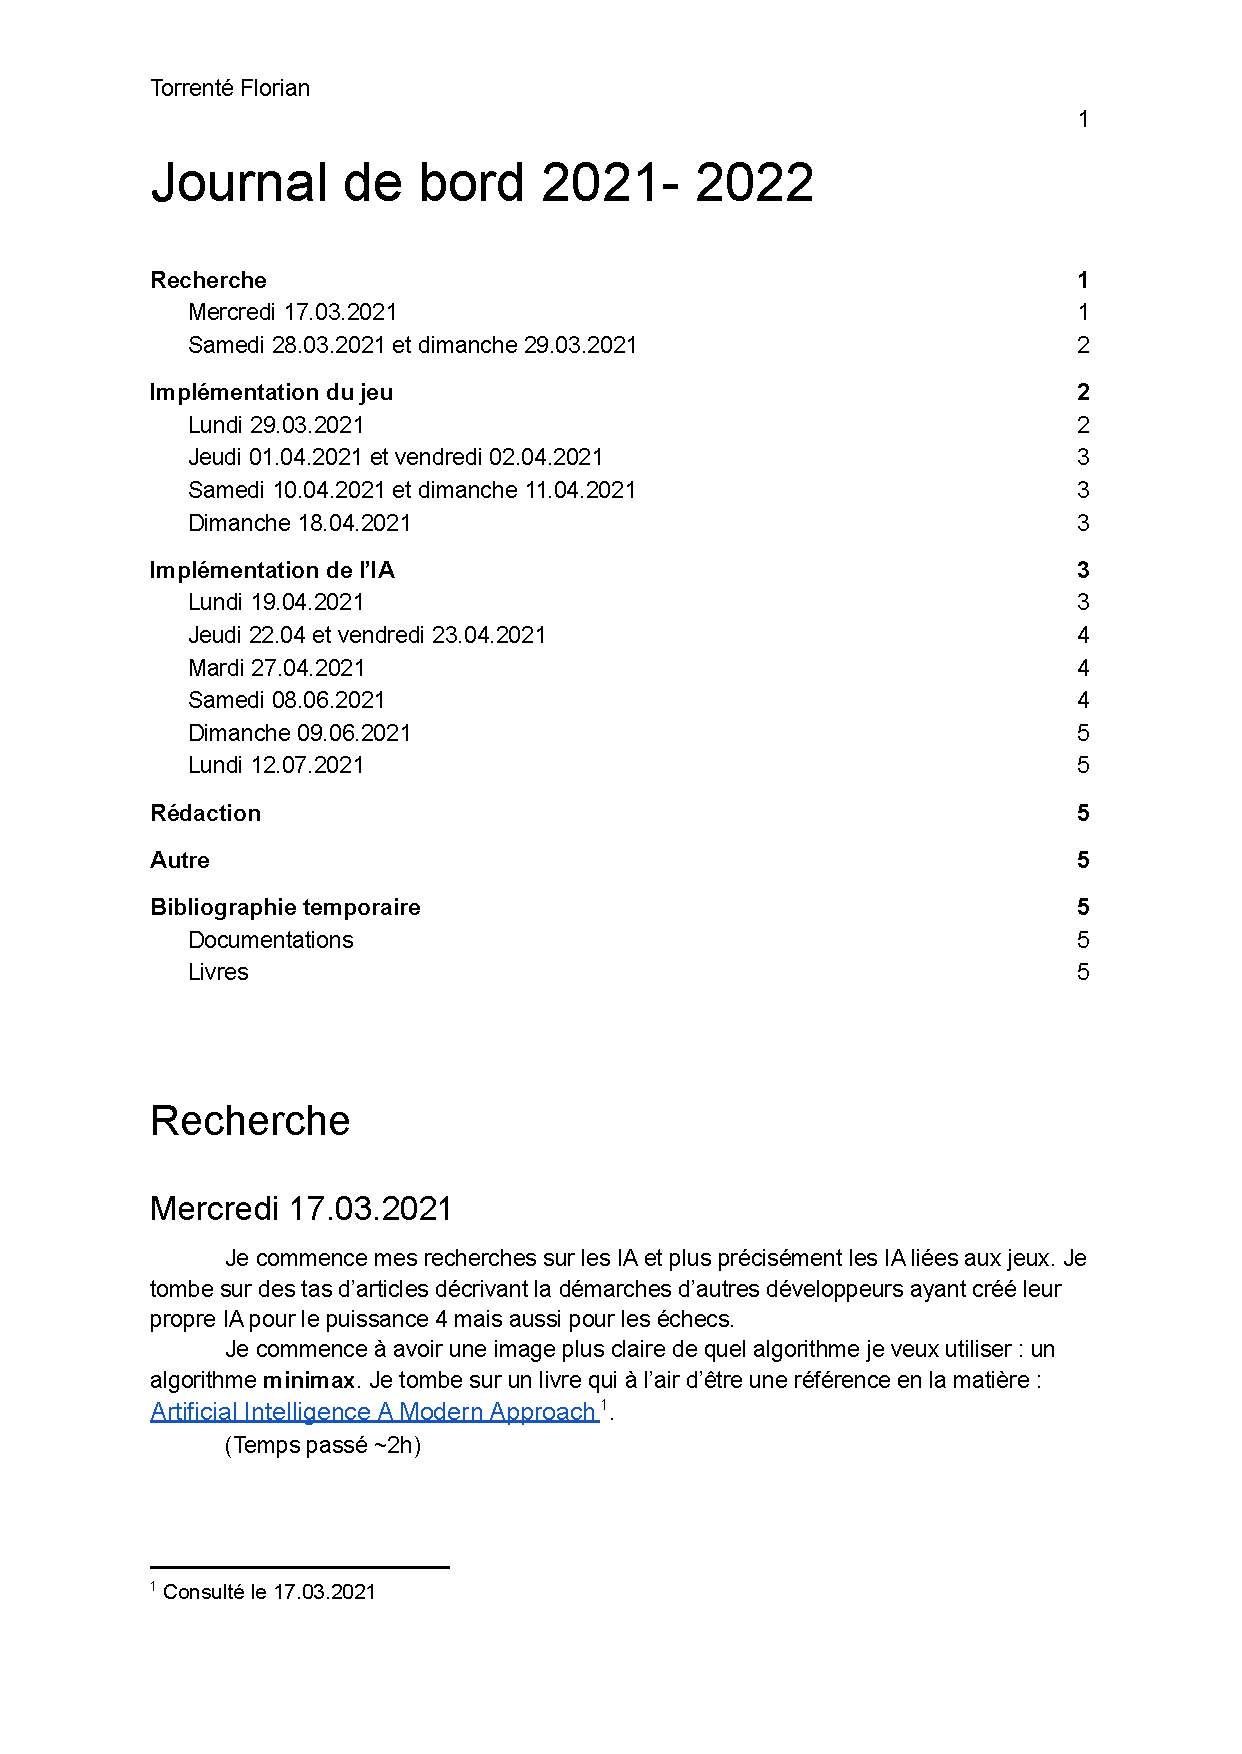
\includepdf[pages=-]{Journal de bord.pdf}

\end{document}